\chapter{Theoretical Foundations}

After a short introduction to the terminology of Big Data, this chapter will discuss the main
characteristics of Big Data Analytics Applications and introduces the concept of stream processing,
which is one of the main characteristics of the popular streaming frameworks Apache Flink and
Apache Kafka. The underlying concepts both of these systems and how they're used in context of
Big Data Analytics will be explained at the end of this chapter.

\section{Big Data}

According to \cite{Marz15} the term “Big Data” is a misleading name since it implies that pre-existing
data is somehow small, which is not true, or that the only challenge is the sheer size of data, which
is just one one them among others. In reality, the term Big Data applies to information that can’t be
processed or analyzed using traditional processes or tools.

In the past decade the amount of data being created is a subject of immense growth. More than
30,000 gigabytes of data are generated every second, and the rate of data creation is only
accelerating.\cite{Marz15}. People create content like blog posts, tweets, social network interactions,
photos, servers continuously log messages, scientists create detailed measurements, permanently.

Through advances in communications technology, people and things are becoming increasingly interconnected.
Generally referred to as machine-to-machine (M2M), interconnectivity is responsible for double-digit year
over year (YoY) data growth rates. Finally, because small integrated components are now affordable, it
becomes possible to add intelligence to almost everything. As an example, a simple railway car has
hundreds of sensors for tracking the state of individual parts and GPS-based data for shipment tracking
and logistics.\cite{Ziko12}

Besides the extremely growing amount of data, an increase in data diversity goes hand in hand.
It comes in its raw and unstructured, semistructured or structured form, which makes processing it in a
traditional relational system impractical or impossible. In \cite{Bitk12} is described, that around
85 percent of the data comes in an unstructured form, but containing valuable information.

Big Data is defined by three characteristics:\cite{Marz15}

\begin{description}
    \item [Volume] The amount of data present is growing because of growing amount of producers,
    e.g. environmental data, financial data, medical data, surveillance data.
    \item [Variety] Data varies in its form, it comes in different formats from different sources.
    \item [Velocity] Data needs to be evaluated and analyzed quickly, which leads to new challenges
    like analysis of large data sets with answers in seconds range, data processing in realtime
    and data generation and transmission at highspeed.
\end{description}


\begin{figure}[H]
	\centering
	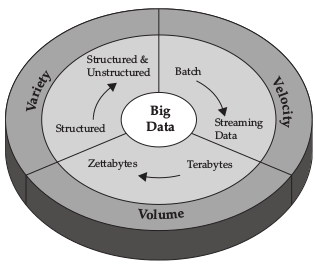
\includegraphics[width=0.7\textwidth]{../images/03-three-vs-of-bigdata.png}
	\caption{The three 'V's of Big Data{\cite{Ziko12}}}
	\label{three-vs-of-bigdata}
\end{figure}

A possible definition for Big Data could be derived as follows:

\textbf{"Big Data refers to the use of large amounts of data from multiple sources with a high processing
speed for generating valuable information based on the underlying data."}

\section{Big Data Analytics Applications}

Big Data Analytics describes the process of collecting, organizing and analyzing large volumes
of data with the aim to discover patterns and other useful information extracted from incoming
data streams \cite{Marz15}. The process of analytics is typically performed using specialized software tools and
applications for predictive analytics, data mining, text mining, forecasting and data optimization.

% Im Vordergrund stehen die Geschwindigkeit der Analyse (Realtime, Near-Realtime) und gleichzeitig die
%einfache Anwendbarkeit, ein ausschlaggebender Faktor beim Einsatz von analytischen Methoden in vielen
%Unternehmensbereichen.

The areas of applications may be extremely diverse and ranges from analysis of financial flows or traffic data, processing
sensor data or environmental monitoring.

%Analytics umfasst die Methoden zur möglichst automatisierten Erkennung und Nutzung von
%Mustern, Zusammenhängen und Bedeutungen. Zum Einsatz kommen u.a. statistische Verfahren,
%Vorhersagemodelle, Optimierungsalgorithmen, Data Mining, Text- und Bildanalytik. Bishe-
%rige Datenanalyse-Verfahren werden dadurch erheblich erweitert.

%Characteristics of Big Data Analytics Applications:
%
%\begin{description}
%    \item [Robustness and fault tolerance] TODO
%    \item [Low latency reads and updates] TODO
%    \item [Generalization] TODO
%    \item [Ad hoc queries] TODO
%\end{description}

\section{Stream Processing}
According to \cite{Klepp16}, stream processing is the real-time processing of data continuously,
concurrently, and in a record-by-record fashion in which data is treated not as static tables
or files, but as a continuous infinite stream of data integrated from both live and historical
sources.

Check \cite{Marz15} S.225 ff.

%Das Streaming-Verarbeitungs-Prinzip steht für die kontinuierliche Verarbeitung von
%Eingangsdaten oder -signalen bei gleichzeitiger kontinuierlicher Bereitstellung von
%Ergebnisdaten oder -signalen. Eingangsdaten liegen oft als Datenstrom vor 28 . Ebenso
%werden die Ausgangsdaten oft als Datenstrom gefordert. Diese Fähigkeit wird im CEP
%genutzt, wo komplexe Regeln die Verarbeitung der Daten steuern.

Benefits of stream processing:

\begin{itemize}
	\item Accessibility: live data can be used while still in motion, before being stored.
	\item Completeness: historical data can be streamed and integrated with live data for more context.
	\item High throughput: high-velocity, high-volume data can be processed with minimal latency.
\end{itemize}

\subsection{Apache Flink}

\subsection{Apache Kafka}

%\subsection{Related work}
%
%\subsubsection{Prometheus}
%
%\subsubsection{Datadog}
%
%\subsubsection{New Relic}
%
%\subsubsection{collectd}

%collectd is a daemon which collects system performance statistics periodically and
%provides mechanisms to store the values in a variety of ways, for example in RRD files.
%
%\subsubsection{collectd}
%
%StatsD is originally a simple daemon developed and  released by Etsy  to aggregate and summarize application metrics.
%With StatsD, applications are to be instrumented by developers using language-specific client libraries. These libraries
%will then communicate with the StatsD daemon using its dead-simple protocol, and the daemon will then generate aggregate
%metrics and relay them to virtually any graphing or monitoring backend.

\section{Summary}